\section{Abläufe}

Während in Kapitel 3 die Interaktion der Hauptkomponenten \emph{Server} und der \emph{RobotUnit} abgehandelt wurden, werden im Folgenden die Abläufe der Use Cases genauer spezifiziert und auch interne Komponentenabläufe beschrieben, im Speziellen die Abläufe innerhalb der \emph{RobotUnit}.
	
	\subsection*{Interaktion bei Ausführung von Use Case 1 \& 2 – \emph{Choose Path around Obstacle \& Drive around Obstacle}}
	Sowohl der UseCase Choose Path Around Obstacle als auch der Use Case Drive AroundObstacle sind beide Teil des Geschäftsprozess DriveToDestionation.  Und wie es schon der Name beschreibt, befindet sich die RobotUnit dabei in einem Fahrvorgang, der vorher konkret mit der Zielposition und er Geschwindigkeit vom Server eingestellt wurde. So reagiert intern seine Software mit dem IDistanceSensor, wenn ein Hindernis um ihn herum auftaucht und dieses mit Hilfe der durch die Sensoren gesammelten Informationen umfahren werden muss. Dabei muss der Roboter ausdrücklich zwischen einem Roboter und einem unbeweglichen Hindernis unterscheiden, um so vorherzubestimmen wie eine optimale Ausweichbewegung aussehen wird. Auch wenn die IDistanceSensor die vollständige Umgebung um den Roboter wahrnehmen kann, bezieht sich dies jedoch primär auf vor dem Roboter liegende Hindernisse. Dieser Prozess ist Bestandteil des Use Case Choose Path around Obstacle und geht dann in den Use Case Drive Around Obstacle über. Der Roboter koordiniert sich dort mit seiner IDrive Komponente und seinen Sensoren, um langsam an einem unbeweglichen Objekt vorbeizufahren. Dabei fährt er immer eine kleine Distanz parallel zur Kante des Obstacles und prüft ob der Weg zur Destination wieder frei ist. Ist dies der Fall nimmt er den Fahrtprozess wieder auf. Erkennen sich zwei Roboter hingegen gegenseitig als Hindernis weichen beide mit Hilfe ihrer IDrive Komponente nach rechts aus, und nehmen den normalen Fahrbetrieb wieder auf. \\
	\begin{figure}[H]
		\centering
		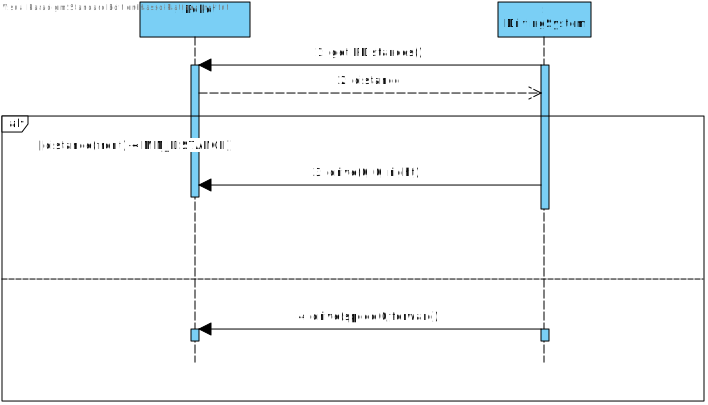
\includegraphics[width=0.75\textwidth]{img/1-Entwurf-8-DriveArroundObstacle}
		\caption{Sequenzdiagramm von \emph{Drive arround Obstacle}}
		\label{Umfahren von statichen Objekten}
	\end{figure}
	
	\subsection*{Interaktion bei Ausführung von Usecase 3 – \emph{ReadSensors}}
In der folgenden Grafik wird der reine Anfrageprozess zwischen Server und der RobotUnit aus Kapitel 3 erweitert. Nach der Anfrage, wird der Robot alle nötigen Informationen nacheinander abfragen: Sowohl die Position als auch die Orientierungsrichtung werden von der INorthStar Komponente zurückgeliefert. Für den Batteriestatus muss die IBatteriekomponente angefragt werden. Erst wenn alle Informationen als Gesamtpaket bereitstehen, können sie an den Server zurückgemeldet werden.
\\
	\begin{figure}[H]
		\centering
		\includegraphics[width=0.75\textwidth]{img/0-Entwurf-8-ReadSens}
		\caption{Sequenzdiagramm von \emph{ReadSensors}}
		\label{ReadSensors}
	\end{figure}
	
	\subsection*{Interaktion bei Ausführung von Use Case 4– \emph{Charging}}
	Auch beim Use Case Charching findet keine Kommunikation mit der Komponente Server statt, dafür allerdings zwischen der RobotUnit und der CharchingStation. Hat der Roboter einen bestimmten kritischen Ladestand erreicht (, den er regelmäßig überprüft), läuft er die CharchingStation Komponente an. Der Ladevorgang triggert automatische, sobald der Roboter die Position der Ladestation erreich hat, und interagiert solange mit ihr bis seine Batterie wieder aufgeladen ist. Innerhalb des Robots werden zum Anfahren der Charching Station die Komponenten IBatterie mit der Position der Robotereigenen Ladestation und IDrive benötigt. Konkret: Wenn IDrive arrived() zurückgibt kann der Ladevorgang begonnen werden.

	
	\begin{figure}[H]
		\centering
		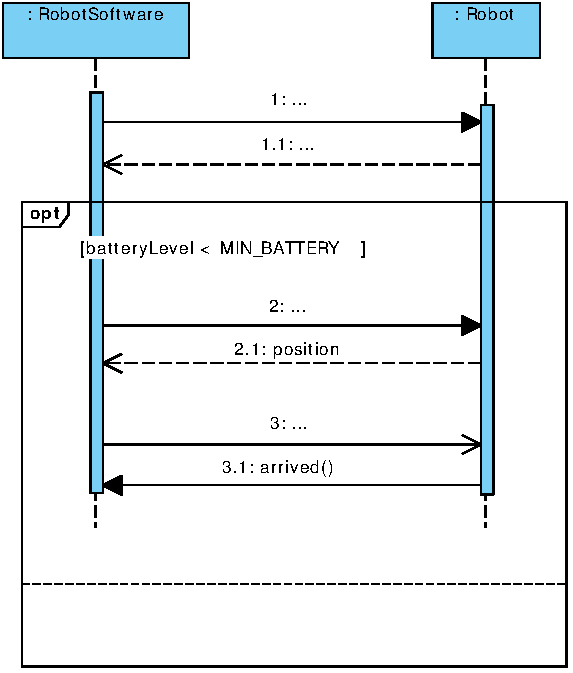
\includegraphics[width=0.75\textwidth]{img/0-Entwurf-8-Charging}
		\caption{Sequenzdiagramm von \texttt{Charging}}
		\label{Charging}
	\end{figure}
